\documentclass{article}

\usepackage{geometry}
\usepackage{booktabs}
\usepackage{multirow}
\usepackage{graphicx}

\graphicspath{{./screenshots/}}
\geometry{margin=1in}


\title{ECE1508 \\Assignment 9}
\author{Iman Tabrizian}
\date{\today}

\begin{document}

\maketitle

\section{Tables for changing the number of features}

In the table below you can find the required parameters for different models.

\begin{table}[htb!]
	\begin{tabular}{ccccccc}
		\toprule
		\multirow{2}{*}{Number of features} & \multicolumn{2}{c}{MLP Model} & \multicolumn{2}{c}{SVR Model} & \multicolumn{2}{c}{LSTM Model} \\ 
		\cmidrule {2-7}
		 & MSE & NMSE & MSE & NMSE & MSE & NMSE  \\
		\midrule
		2 & 0.0030 & 1.3362 & 0.00124 & 0.53860 & 0.000929 & 0.401565 \\
		\midrule
		3 & 0.002478 & 1.070945 & 0.0013970 & 0.603586 &  0.0009302 &  0.4018888 \\
		\midrule
		4 & 0.002278 & 0.984495 & 0.001482 & 0.640301 & 0.0009307 & 0.402099 \\
		\midrule
		5 & 0.00289005 & 1.2485928 & 0.001585 & 0.685133 & 0.000932 & 0.402881 \\
		\midrule
		6 & 0.00228 & 0.985315 & 0.001719 & 0.7426875 & 0.000960 & 0.415013 \\
		\midrule
		7 & 0.002970 & 1.283182 & 0.0017731 & 0.766035 & 0.0009713 & 0.4196461 \\
		\midrule
		8 & 0.002778 & 1.20036 & 0.0018228 & 0.7875077 & 0.0009597 & 0.414649 \\
		\midrule
		9 & 0.00268616 & 1.1605072 & 0.0018670 & 0.8066385 & 0.00097864 & 0.4228032 \\
		\midrule
		10 & 0.0029216 & 1.2622376 & 0.0018720 & 0.808783 & 0.000967 & 0.4181357  \\
		\bottomrule
	\end{tabular}
	\caption{Table of Results (for residuals time-series)}
\end{table}


\begin{table}[htb!]
	\begin{tabular}{ccccccc}
		\toprule
		\multirow{2}{*}{Number of features} & \multicolumn{2}{c}{MLP Model} & \multicolumn{2}{c}{SVR Model} & \multicolumn{2}{c}{LSTM Model} \\ 
		\cmidrule {2-7} & MSE & NMSE & MSE & NMSE & MSE & NMSE  \\
		\midrule
		2 & 68225.57212 & 0.171056 & 27498.95825 & 0.068946 & 20502.16173 & 0.0514035 \\
		\midrule
		3 & 54677.739207 & 0.1370894 & 30816.455177 & 0.077263 & 20518.6681 & 0.051444 \\
		\midrule
		4 & 50264.012671 & 0.126023 & 32690.94230 & 0.081963 & 20529.4436 & 0.0514719 \\
		\midrule
		5 & 63747.635962 & 0.159829 & 34979.8985 & 0.087702 & 20569.35681 & 0.051572 \\
		\midrule
		6 & 50305.83902 & 0.126128 & 37918.34910 & 0.095069 & 21188.76456 & 0.0531250 \\
		\midrule
		7 & 65513.63663 & 0.164257 & 39110.38633 & 0.098058 & 21425.27793 & 0.053718 \\
		\midrule
		8 & 61285.52556 & 0.153656 & 40206.6670 & 0.100807 & 21170.1896 & 0.053078 \\
		\midrule
		9 & 59250.3738 & 0.1485541 & 41183.39976 & 0.1032561 & 21586.46805 & 0.054122 \\
		\midrule
		10 & 64444.27925 & 0.161576 & 41292.90400 & 0.103530 & 21348.16552 & 0.0535246 \\
		\bottomrule
	\end{tabular}
	\caption{Table of Results (for original time-series)}
\end{table}

\begin{table}[htb!]
	\begin{tabular}{cccc}
		\toprule
		Number of Features & MLP Model time (sec) & SVR Model time (sec) & LSTM Model time (sec) \\
		\midrule 
		2 & 0.1230 & 0.0163 & 32.4487 \\ 
		\midrule
		3 & 0.1482 & 0.0135 & 33.1699 \\
		\midrule
		4 & 0.1136 & 0.0134 & 37.8190 \\
		\midrule
		5 & 0.1621 & 0.0145 & 37.0023 \\
		\midrule
		6 & 0.1623 & 0.0143 & 33.7526 \\
		\midrule
		7 & 0.1253 & 0.0176 & 38.1295 \\
		\midrule
		8 & 0.0936 & 0.0139 & 34.2890 \\
		\midrule
		9 & 0.1786 & 0.0135 & 36.2493 \\
		\midrule
		10 & 0.0957 & 0.0142 & 36.1076 \\
		\bottomrule
	\end{tabular}
	\caption{Table of Results (training time)}
\end{table}

\section{Tables for changing the number of training and test samples}

You can find the results in table 4, 5 and 6.

\begin{table}[htb!]
	\centering
	\begin{tabular}{p{2cm} p{2cm} p{2cm} p{2cm} p{2cm}}
		\toprule
		Number of Training Samples & Number of Test Samples & MLP Model (NMSE) & SVR Model (NMSE) & LSTM Model (NMSE) \\
		\midrule
		100 & 100 & 1.689960 & 1.00217713 & 0.4138247 \\
		\midrule
		300 & 100 & 1.2698733 & 0.727063  & 0.414500909 \\
		\midrule
		500 & 150 & 1.43755887 & 0.6953694 & 0.42535019 \\
		\midrule
		700 & 100 & 1.3009608 & 0.6851336 & 0.40292855 \\
		\midrule
		800 & 250 & 1.33861230 & 0.63293716 & 0.4201770 \\
		\midrule
		1000 & 250 & 0.794297 & 0.63445184 & 0.42180600 \\
		\midrule
		1500 & 500 & 0.96651828 & 0.5778822 & 0.4480015 \\
		\midrule
		2000 & 300 & 1.03940 & 0.5402691 & 0.4445546 \\
		\midrule
		2000 & 700 & 1.055143255 & 0.51158609 & 0.42775509 \\
		\midrule
		2000 & 1000 & 0.770215069 & 0.501095751 & 0.4175145106 \\
		\bottomrule
	\end{tabular}
	\caption{Table of Results (error for residual time-series)}
\end{table}

\begin{table}[htb!]
	\centering
	\begin{tabular}{p{2cm} p{2cm} p{2cm} p{2cm} p{2cm}}
		\toprule
		Number of Training Samples & Number of Test Samples & MLP Model (NMSE) & SVR Model (NMSE) & LSTM Model (NMSE) \\
		\midrule
		100 & 100 & 0.2163283 & 0.1282866 & 0.0529728 \\
		\midrule
		300 & 100 & 0.16255385 & 0.0930699 & 0.0530593 \\ 
		\midrule
		500 & 150 & 0.06214910 & 0.03006248 & 0.018388905 \\
		\midrule
		700 & 100 & 0.1665332 & 0.087702533 & 0.05157804 \\
		\midrule
		800 & 250 & 0.03828910 & 0.01810426 & 0.0120185676 \\
		\midrule
		1000 & 250 & 0.02271976  & 0.018147593 & 0.012065161 \\
		\midrule
		1500 & 500 & 0.0193519 & 0.01157052 & 0.00897001 \\
		\midrule
		2000 & 300 & 0.02414774 & 0.012551687 & 0.01032801 \\
		\midrule
		2000 & 700 & 0.01862322 &  0.00902947 & 0.007549857 \\
		\midrule
		2000 & 1000 & 0.0136075 & 0.00885297 & 0.00737632 \\
		\bottomrule
	\end{tabular} \caption{Table of Results (error for original time-series)}
\end{table}

\begin{table}[htb!]
	\centering
	\begin{tabular}{p{2cm} p{2cm} p{2cm} p{2cm} p{2cm} p{2cm}}
		\toprule
		Number of Training Samples & Number of Test Samples & MLP Model time (sec) & SVR Model time (sec) & LSTM Model time (sec) \\
		\midrule
		100 & 100 & 0.0478 & 0.0046 & 11.3590 \\
		\midrule
		300 & 100 & 0.1562 & 0.0047 & 13.7445 \\
		\midrule
		500 & 150 & 0.1715 & 0.0055 & 18.3428 \\
		\midrule
		700 & 100 & 0.0898 & 0.0066 & 19.4059 \\
		\midrule
		800 & 250 & 0.0964 & 0.0080 & 23.1421 \\
		\midrule
		1000 & 250 & 0.0893 & 0.0087 & 26.9709 \\
		\midrule
		1500 & 500 & 0.1268 & 0.0145 & 38.3500 \\
		\midrule
		2000 & 300 & 0.2651 & 0.0254 & 41.3337 \\
		\midrule
		2000 & 700 & 0.3536 & 0.0244 & 47.1275 \\
		\midrule
		2000 & 1000 & 0.1729 & 0.0246 & 49.6868 \\
		\bottomrule
	\end{tabular}
	\caption{Table of Results (training time)}
\end{table}

\section{Changing parameters of the model}

\begin{table}[htb!]
	\centering
	\begin{tabular}{p{2cm} p{2cm} p{2cm}}
		\toprule
		Kernel & SVR Model (NMSE) & SVR Model time (sec)  \\
		\midrule
		rbf & 0.010760054 & 0.0138 \\
		\midrule
		linear & 0.0102815448 & 0.0120 \\
		\midrule
		poly & 0.02005216 & 0.0155 \\
		\midrule
		sigmoid & 0.01157052 & 0.0141 \\
		\bottomrule
	\end{tabular}
	\caption{Table of Results (training time)}
\end{table}

\begin{table}[htb!]
	\centering
	\begin{tabular}{p{2cm} p{2cm} p{2cm}}
		\toprule
		Number of Neurons & LSTM Model (NMSE) & LSTM Model time (sec)  \\
		\midrule
		100 & 0.0096152 & 5.1772 \\
		\midrule
		200 & 0.0090583 & 9.0979 \\
		\midrule
		300 & 0.0089833 & 13.7074 \\
		\midrule
		400 & 0.0089717 & 20.9778 \\
		\midrule
		500 & 0.0089696 & 26.7895 \\
		\midrule
		600 & 0.0089702 & 35.0587 \\
		\midrule
		700 & 0.0089704 & 49.3502 \\
		\midrule
		800 & 0.008971175 & 58.2411 \\
		\midrule
		900 & 0.008971458 & 69.0857 \\
		\bottomrule
	\end{tabular}
	\caption{Table of Results (training time)}
\end{table}

\begin{enumerate}
	\item SVR Model \\
		The result of SVR model can be found in table 7
	\item LSTM Model \\
		The result of the LSTM model can be found in table 8
\end{enumerate}

\pagebreak

\section{Find the optimal number of features}

\begin{enumerate}
	\item \textbf{DATA} and \textbf{SCALED} data are both LRD as you can see in the figure 1 but \textbf{DIFF} is SRD.
	\item You can find the values below
		\begin{enumerate}
			\item 2
			\item 3
			\item 4
			\item 5
		\end{enumerate}
\end{enumerate}

\begin{figure}[htb!]
	\centering
	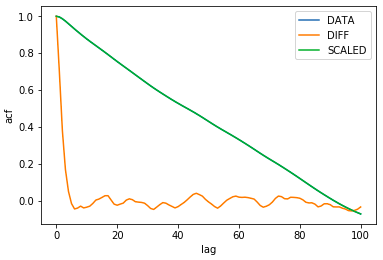
\includegraphics{acf-graph}
	\caption{Graph of 3 versions of ACF values}
\end{figure}

\pagebreak

\section{Find the optimal number of features}

\begin{table}[htb!]
	\centering
	\begin{tabular}{p{2cm} p{2cm} p{2cm} p{2cm} p{2cm}}
		\toprule
		Number of Training Samples & Number of Test Samples & MLP Model (NMSE) & SVR Model (NMSE) & LSTM Model (NMSE) \\
		\midrule
		100 & 100 & 2.401500277 & 0.221028781 & 0.48854918 \\
		\midrule
		300 & 100 & 0.52043904 & 0.1418267760 & 0.267770564 \\
		\midrule
		500 & 150 & 0.271403002 & 0.0432134286 & 0.13468817 \\
		\midrule
		700 & 100 & 0.898979734 & 0.1133347042 & 0.438534549 \\
		\midrule
		800 & 250 & 0.204156149 & 0.029631597 & 0.0819993948 \\
		\midrule
		1000 & 250 & 0.23636296 & 0.02857671 & 0.08829583 \\
		\midrule
		1500 & 500 & 0.07355060 & 0.0170794 & 0.066361683 \\
		\midrule
		2000 & 300 & 0.24682069 & 0.020613206 & 0.0709812743 \\
		\midrule
		2000 & 700 & 0.12266811 & 0.01262712643 & 0.054285968 \\
		\midrule
		2000 & 1000 & 0.0910693 &  0.0123333436 & 0.0585874751 \\
		\bottomrule
	\end{tabular}
	\caption{Table of Results (error for scaled time-series)}
\end{table}

\begin{table}[htb!]
	\centering
	\begin{tabular}{p{2cm} p{2cm} p{2cm} p{2cm} p{2cm}}
		\toprule
		Number of Training Samples & Number of Test Samples & MLP Model (NMSE) & SVR Model (NMSE) & LSTM Model (NMSE) \\
		\midrule
		100 & 100 & 2.4015002772 & 0.2210287814 & 0.48854920176 \\
		\midrule
		300 & 100 & 0.520439049 & 0.14182677 & 0.267770536 \\ 
		\midrule
		500 & 150 & 0.271403002 & 0.0432134286 & 0.1346881749 \\
		\midrule
		700 & 100 & 0.89897973 & 0.1133347042 & 0.43853452 \\
		\midrule
		800 & 250 & 0.204156149 & 0.02963159 & 0.08199940 \\
		\midrule
		1000 & 250 & 0.23636296  & 0.028576715 & 0.08829582 \\
		\midrule
		1500 & 500 & 0.07355060 & 0.0170794986 & 0.066361684 \\
		\midrule
		2000 & 300 & 0.24682069 & 0.0206132069 & 0.0709812 \\
		\midrule
		2000 & 700 & 0.12266811 & 0.0126271264 & 0.05428596 \\
		\midrule
		2000 & 1000 & 0.09106933 & 0.01233334 & 0.0585874 \\
		\bottomrule
	\end{tabular} \caption{Table of Results (error for original time-series)}
\end{table}

\begin{table}[htb!]
	\centering
	\begin{tabular}{p{2cm} p{2cm} p{2cm} p{2cm} p{2cm} p{2cm}}
		\toprule
		Number of Training Samples & Number of Test Samples & MLP Model time (sec) & SVR Model time (sec) & LSTM Model time (sec) \\
		\midrule
		100 & 100 & 0.0979 & 0.0044 & 10.9229 \\
		\midrule
		300 & 100 & 0.3224 & 0.0065 & 14.6880 \\
		\midrule
		500 & 150 & 0.1789 & 0.0091 & 17.0320 \\
		\midrule
		700 & 100 & 0.3709 & 0.0119 & 20.9940 \\
		\midrule
		800 & 250 & 0.7287 & 0.0150 & 23.7504 \\
		\midrule
		1000 & 250 & 0.3730 & 0.0163 & 28.4276 \\
		\midrule
		1500 & 500 & 0.5067 & 0.0320 & 38.3334 \\
		\midrule
		2000 & 300 & 0.3128 & 0.0655 & 44.8276 \\
		\midrule
		2000 & 700 & 0.7275 & 0.0653 & 46.7937 \\
		\midrule
		2000 & 1000 & 0.9362 & 0.0679 & 50.3620 \\
		\bottomrule
	\end{tabular}
	\caption{Table of Results (training time)}
\end{table}
\end{document}
